\begin{figure}
  \centering
  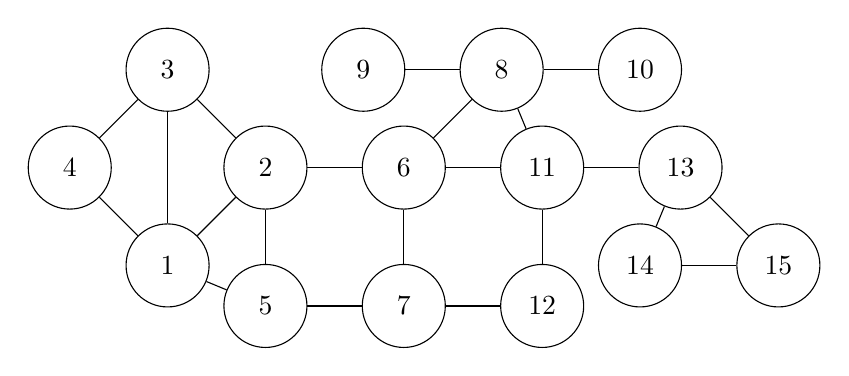
\begin{tikzpicture}[auto, node distance=5em, main node/.style={circle, draw, minimum size=3em}]
    \node (1) [main node] {1};
    \node (2) [main node, above right of=1] {2};
    \node (3) [main node, above left of=2] {3};
    \node (4) [main node, above left of=1] {4};
    \node (5) [main node, below of=2] {5};
    \node (6) [main node, right of=2] {6};
    \node (7) [main node, right of=5] {7};
    \node (8) [main node, above right of=6] {8};
    \node (9) [main node, left of=8] {9};
    \node (10) [main node, right of=8] {10};
    \node (11) [main node, right of=6] {11};
    \node (12) [main node, right of=7] {12};
    \node (13) [main node, right of=11] {13};
    \node (14) [main node, below right of=11] {14};
    \node (15) [main node, right of=14] {15};

    \path[every node]
    (1) edge (2) edge (3) edge (4) edge (5)
    (2) edge (3) edge (5) edge (6)
    (3) edge (4)
    (5) edge (7)
    (6) edge (7) edge (8) edge (11)
    (7) edge (12)
    (8) edge (9) edge (10) edge (11)
    (11) edge (12) edge (13)
    (13) edge (14) edge (15)
    (14) edge (15)
    ;
  \end{tikzpicture}

  \caption{Graph $G$}\label{fig:bridgegraph}
\end{figure}